\documentclass[12pt]{article}
\usepackage{amsmath}
\usepackage{graphicx}
\usepackage{hyperref}
\usepackage[utf8]{inputenc}
\usepackage[T1]{fontenc}
\usepackage[polish]{babel}

\author{Aleksander Głowacki}
\title{Sprawozdanie nr 3}
\date{27.11.2022}

\begin{document}

\maketitle

\tableofcontents

\section{Zadanie 1.}


\subsection{Opis problemu}
Rozwiązanie równania postaci $ f(x) = 0 $ metodą bisekcji.

\subsection{Sposób rozwiązania}
Szukamy miejsca zerowego funkcji na danym przedziale: $(a,b)$. \newline Jeżeli funkcja
jest ciągła na przedziale i $sign(f(a)) \neq sign(f(b))$ to znaczy, że istnieje 
miejsce zerowe funkcji na tym przedziale. (Twierdzenie Darboux o wartości pośredniej)\newline
Jego przybliżeniem będzie wartość $c$ równo pomiędzy $a$ i $b$.\newline
\begin{figure}[h]
    \caption{ilustracja metody poławiania}
    \centering
    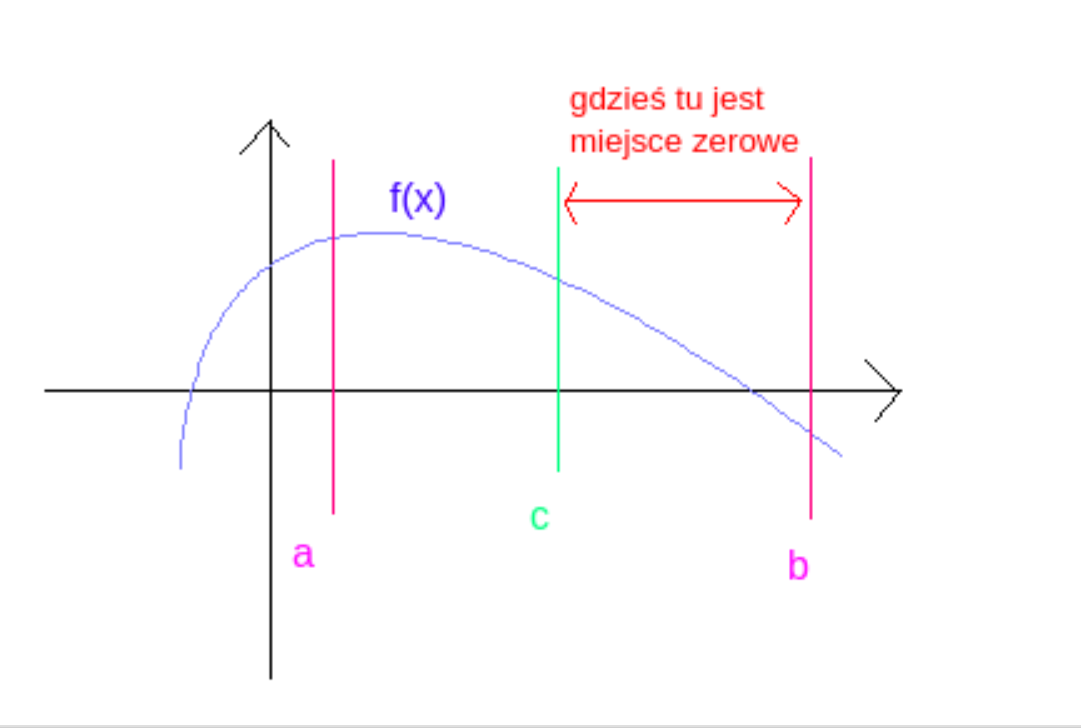
\includegraphics[width=12cm]{polawianie.png}
\end{figure}
Jeżeli chcemy uzyskać lepsze przybliżenie to spradzamy na którym z dwóch 
przedziałów $(a,c)$ i $(c,b)$ funkcja zmienia znak ten przedział rozważamy, bo w nim występuje miejsce zerowe.
\newline Powyższy schemat powtarzamy aż do uzyskania pożądanej dokładności.
Delta określa szerokość przedziału na którym wystęþuje przecięcie funkcji $f(x)$ 
z osią $OX$, natomiast epsilon bada "wysokość" czyli wartość funkcji w znalezionym punkcie - to 
jak bardzo odbiega od zera.

\section{Zadanie 2.}

\subsection{Opis problemu}
Rozwiązanie równania postaci $ f(x) = 0 $ metodą stycznych.
W tym problemie konieczna jest znajomość pochodnej badanej funkcji.
W danych wejściowych konieczne jest również jakiekolwiek początkowe przybliżenie $x0$

\subsection{Sposób rozwiązania}
Szukamy miejsca zerowego na podstawie stycznej do wykresu funkcji.\newline
Styczna ma jeden punkt wspólny z krzywą - początkowo oznaczmy go $(x0, f(x0))$.
Miejsce przecięcia stycznej z osią OX wyznacza przybliżenie szukanego miejsca zerowego $f(x)$. \newline
Aby uzyskać dokładniejszy wynik powtarzamy wyznaczenie stycznej, tym razem od punktu, który przed cheilą wyznaczyliśmy, 
na wykresie $f(x)$. \newline 
Wzór na styczną: 
\begin{center}
    $y = f'(x_{0})(x - x_{0}) + f(x_{0})$
\end{center}
Podstawiamy $y := 0$ aby otrzymać $x$
\begin{center}
    $0 = f'(x_0)(x) - f'(x_0)(x_0) + f(x_0)$
\end{center}
\begin{center}
    $x =  \frac{(f'(x_0)(x_0) - f(x_0))}{f'(x_0)}$
\end{center}
\begin{center}
    $x = x_0 - \frac{f(x_0)}{f'(x_0)}$
\end{center}
Wykonując iteracyjnie algorytm wyznaczania siecznych i miejsc ich przecięcia z osią X otrzymujemy coraz dokładniejsze 
przybliżenie miejsca zerowego fukncji $f(x)$
\begin{figure}[htp]
    \caption{źródło: https://kmim.wm.pwr.edu.pl/myszka/dydaktyka/informatyka-i/laboratoriumprojekt/laboratorium-6-funkcje-metoda-newtona-raphsona/}
    \centering
    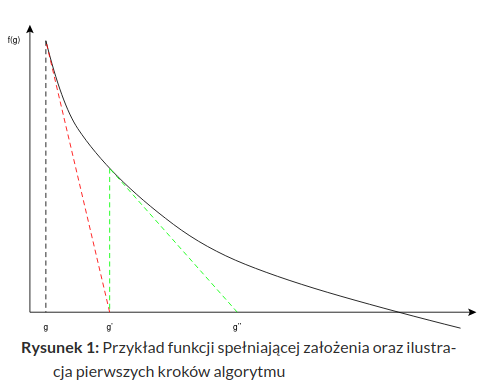
\includegraphics[width=12cm]{st1.png}
\end{figure}
\newpage
\section{Zadanie 3.}

\subsection{Opis problemu}
Rozwiązanie równania postaci $ f(x) = 0 $ metodą siecznych.
Do rozwiązania problemu musimy zapewnić dwa punkty na których będziemy kłaść sieczną względem
funkcji $f(x)$. Czyli po prostu krańce przedziału tak jak w metodzie bisekcji.

\subsection{Sposób rozwiązania}
Wyznaczamy równanie prostej przechodzącej przez dwa punkty na wykresie funkcji:
$(x_0, f(x_0))$ i $(x_1, f(x_1))$. Znajdujemy r - miejsce przecięcia z osią OX. To właśnie jest
nasze wstępne przybliżenie pierwiastka.\newline
Następnie działamy w pętli aż do uzyskania odpowiedniej dokładności lub limitu iteracji:\newline
Badamy który z przedziałów $(x0, r) i (r, x1)$ zawiera miejsce zerowe - zmiana znaku wartości na krańcach przedziału.
Odpowiednio oznaczamy nowy przedział i nowe punkty do położenia siecznej i szukamy nowego przecięcia siecznej z osią OX.
\newline
\begin{figure}[!h]
    \caption{ilustracja metody siecznych}
    \centering
    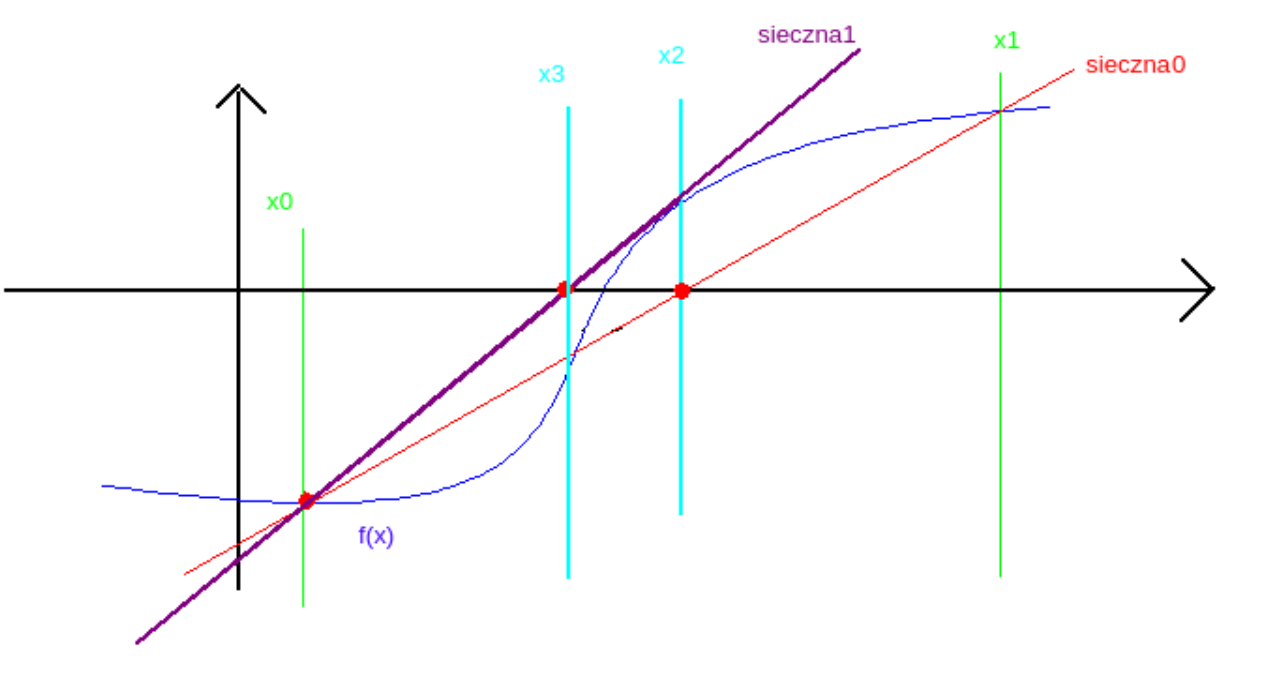
\includegraphics[width=14cm]{sieczne.png}
\end{figure}
Wzór na sieczną:
\begin{center}
    $(y - f(x_0)(x_1 - x_0) - (f(x_1) - f(x_0))(x - x_0))$
\end{center}
Podstawiamy $y := 0$ aby znaleźć miejsce przecięcia z OX.
\begin{center}
    $(f(x_1) - f(x_0))(x_0)-f(x_0)(x_1 - x_0) = (f(x_1) - f(x_0))(x)$
\end{center}
\begin{center}
    $x = x_0 - f(x_0) \frac{x_1 - x_0}{f(x_1) - f(x_0)}$
\end{center}
\newpage
\newpage
\section{Zadanie 4.}

\subsection{Opis problemu}
Znalezienie rozwiązania równania:
\begin{center}
    $sin(x) - (\frac{x}{2})^2$
\end{center}
za pomocą trzech różnych metod.
\subsection{Sposób rozwiązania}
Użycie oprogramowanych funkcji dla danych z zadania i wyświetlenie wynikow.
\newpage
\subsection{Wyniki}
\begin{table}[h]
    \caption{porównanie metod wyznaczania pierwiastka}
    \label{epsilblankon}
    %\centering
    \begin{tabular}{|l|l|l|l|l|}
        \hline 
        \textbf{metoda} & \textbf{r} & \textbf{v } & \textbf{it } & \textbf{err}\\
        \hline
        \textbf{Bisekcja} & 1.9337539672851562 & -2.7027680138402843e-7 & 16 & 0\\
        \hline
        \textbf{Styczne} & 1.933753779789742 & -2.2423316314856834e-8 & 4 & 0\\
        \hline
        \textbf{Sieczne} & 1.9337509005356321 & 3.783706985283075e-6 & 4 & 0\\
        \hline
    \end{tabular} 
\end{table}

\subsection{Wnioski}
\begin{enumerate}
    \item Wszystkie metody są skuteczne, ponieważ odnalazły pierwiastek w danej dokładności.
    \item W testowanym przypadku metoda Newtona jest najskuteczniejsza, ponieważ wykonała najmniej iteracji.
\end{enumerate}

\section{Zadanie 5.}

\subsection{Opis problemu}
Szukanie miejsca przecięcia funkcji $f(x) = e^x \hspace{0.5cm}i\hspace{0.5cm} g(x) = 3*x$
\subsection{Sposób rozwiązania}
Porównujemy zadane funkcje ze sobą, jedną z nich przerzucamy na drugą stronę i otrzymujemy równanie
postaci $f(x) - g(x) = 0$ gdzie lewa strona jest nową funkcją, której pierwiastków szukamy.
Miejsca przecięcia będą prwadopodobnie dwa, ewentualnie jedno lub wcale.
Na początkowe przedziały wziąłem $(-10,1)$ i $(1,10)$
\newpage
\subsection{Wyniki}
\begin{table}[h]
    \caption{przecięcia funkcji}
    \label{pierwiastki}
    %\centering
    \begin{tabular}{|l|l|l|l|l|}
        \hline 
        \textbf{ } & \textbf{r} & \textbf{v } & \textbf{it } & \textbf{err}\\
        \hline
        \textbf{Bisekcja1} & 1.5121002197265625 & -5.274503124397256e-5 & 16 & 0\\
        \hline
        \textbf{Bisekcja2} & 0.618988037109375 & 8.371583772359692e-5 & 15 & 0\\
        \hline
    \end{tabular} 
\end{table}
\subsection{Wnioski}
Dokładność wyników zależy od początkowo ustalonego przedziału. W najgorszym wypadku wyniku nie będzie.
Dalsze błędy zaokrągleń wynikają z dzielenia przedziału na pół - im szerszy przedział początkowy, tym więcej błędów może narosnąć.
Nie są one jednak poważne, bo wyniki i tak znalazły się w kilkunastu iteracjach. 

\section{Zadanie 6.}

\subsection{Opis problemu}
Znalezienie pierwiastków funkcji: 
\begin{center}
    $f(x) = e^{1-x} \hspace*{2cm} g(x) = x * e^{-x}$
\end{center}
metodami bisekcji, stycznych i siecznych dla dokładności rzędu $10^{-5}$
\subsection{Analiza}

$lim_{x\rightarrow \infty}\;f(x)\;=\; -1$\newline
$lim_{x\rightarrow \infty}\;g(x)\;=\; 0$\newline
Jeżeli szukamy przecięcia funkcji z osią OX gdy funkcja jest zbieżna do tej osi,
to mamy duży problem. W granicy do nieskończoności funkcja osiąga wartości 
coraz bliższe zera aż w końcu kończy się precyzja arytmetyki i komputer
będzie ustawiał te wartości dookoła zera, co jest niezgodne z prawdą.
Możemy mieć sytuację, że funkcja zbiega do 0, a nigdy go nie osiąga, a mimo tego
na komputerze możemy to 0 otrzymać w wyniku skończonej precyzji arytmetyki.
\subsection{Wyniki}

\begin{table}[h]
    \caption{Metoda bisekcji dla dokładności rzędu $10^{-5}$}
    \label{bisekcja}
    %\centering
    \begin{tabular}{|l|l|l|l|l|l|}
        \hline 
        \textbf{funkcja} & \textbf{range} & \textbf{root} & \textbf{f(root)} & \textbf{it } & \textbf{err}\\
        \hline
        \textbf{f} & $(-1, 1000)$ & 0.9999999443534762 & 5.5646525387587076e-8 & 32 & 0\\
        \hline
        \textbf{g} & $(-1, 1000)$ & 499.5 & 5.867347112928062e-215 & 1 & 0\\
        \hline
        \textbf{f} & $(-10, 10)$ & 0.9999999403953552 & 5.960464655174746e-8 & 26 & 0\\
        \hline
        \textbf{g} & $(-10, 10)$ & 0.0 & 0.0 & 1 & 0\\
        \hline
        \textbf{f} & $(-10, -1)$ & Nothing & Nothing & Nothing & 1\\
        \hline
        \textbf{g} & $(-10, -1)$ & Nothing & Nothing & Nothing & 1\\
        \hline
        \textbf{f} & $(-1, 2)$ & 1.0000000596046448 & -5.9604642999033786e-8 & 24 & 0\\
        \hline
        \textbf{g} & $(-1, 2)$ & -5.960464477539063e-8 & -5.960464832810441e-8 & 24 & 0\\
        \hline
    \end{tabular} 
\end{table}

\begin{table}[h]
    \caption{Metoda Newtona dla dokładności rzędu $10^{-5}$}
    \label{Newton}
    %\centering
    \begin{tabular}{|l|l|l|l|l|l|}
        \hline 
        \textbf{funkcja} & \textbf{x0} & \textbf{root} & \textbf{f(root)} & \textbf{it } & \textbf{err}\\
        \hline
        \textbf{f} & $ -5.0 $ & 0.9999999998809204 & 1.1907963504143027e-10 & 10 & 0\\
        \hline
        \textbf{g} & $ -5.0 $ & -8.215721693760581e-11 & -8.215721694435562e-11 & 11 & 0\\
        \hline
        \textbf{f} & $ 2.5 $ & 0.9999999999788638 & 2.1136203898208805e-11 & 7 & 0\\
        \hline
        \textbf{g} & $ 2.5 $ & 19.84810470417909 & 4.7620800660145274e-8 & 15 & 0\\
        \hline
        \textbf{f} & $ 10.0 $ & Nothing & Nothing & Nothing & 1\\
        \hline
        \textbf{g} & $ 10.0 $ & 19.70579463139675 & 5.450998750038715e-8 & 9 & 0\\
        \hline
        \textbf{f} & $ 1.0 $ & 1.0 & 0.0 & 0 & 0\\
        \hline
        \textbf{g} & $ 1.0 $ & Nothing & Nothing & Nothing & 2\\
        \hline
    \end{tabular} 
\end{table}
\begin{table}[h]
    \caption{Metoda siecznych dla dokładności rzędu $10^{-5}$}
    \label{sieczne}
    %\centering
    \begin{tabular}{|l|l|l|l|l|l|}
        \hline 
        \textbf{funkcja} & \textbf{(x0, x1)} & \textbf{root} & \textbf{f(root)} & \textbf{it } & \textbf{err}\\
        \hline
        \textbf{f} & $ (0.0, 2.0) $ & 1.0000000767640695 & -7.676406654777423e-8 & 19 & 0\\
        \hline
        \textbf{g} & $ (0.0, 2.0) $ & 0.0 & 0.0 & 1 & 0\\
        \hline
        \textbf{f} & $ (-20.0, 30.0) $ & Nothing & Nothing & Nothing & 1\\
        \hline
        \textbf{g} & $ (-20.0, 30.0) $ & 30.0 & 2.8072868906520526e-12 & 1 & 0\\
        \hline
        \textbf{f} & $ (-2.0, 3.0) $ & 1.0000000897951176 & -8.979511356699277e-8 & 102 & 0\\
        \hline
        \textbf{g} & $ (-2.0, 3.0) $ & 8.891398861621269e-8 & 8.891398071051567e-8 & 147 & 0\\
        \hline
        \textbf{f} & $ (2.0, 5.0) $ & 1.0000017595679251 & -1.7595663771574621e-6 & 247 & 0\\
        \hline
        \textbf{g} & $ (2.0, 5.0)$ & Nothing & Nothing & Nothing & 1\\
        \hline
    \end{tabular} 
\end{table}

\newpage
\subsection{Wnioski}
\begin{enumerate}
    \item Algorytmy mają swoje wady - głównie to że znajdują rzekome pierwiastki gdy funkcja zbiega 
    do zera i w wyniku błędów arytmetyki wskazują na przecięcia.
    \item Dobierając odpowiednio początkowe przybliżenia można jednak uzyskać prawidłowe wyniki.
    \item Algorytmy nie są złe, błedy wynikają z ograniczeń komputera a nie samych algorytmów.
\end{enumerate}
\subsection{Odpowiedzi na pytania}

Czy można wybrać początkowe przybliżenie $x0 = 1$ dla $g(x)$?\newline
Odp: Nie, ponieważ zwracam wtedy błąd dzielenia przez 0.
\newline
Co się stanie gdy w metodzie Newtona wybiorę $ x0 >> 1 $ dla $f(x)$?
\newline
Odp: Nie dostanę wyniku  w zadanej precyzji, bo będzie zbyt dużo iteracji.
Dla dużych x to pochodna pada zbyt blisko zera i wtedy też sie psuje i dostaję inny kod błędu.
\newline
Co się stanie gdy dla $g(x)$ podam $x0 > 1$?
\newline
Odp: Znajdę fikcyjne pierwiastki, ponieważ w wyniku skończonej precyzji arytmetyki otrzymuję
zakłamania gdy funkcja zbiega do zera. Metoda Newtona znajduje przecięcia które
się pojawiły w wyniku błędów arytmetyki.

\end{document}
